\documentclass[aspectratio=169]{beamer}
%% For 4:3 aspect ratio:
%% \documentclass{beamer}
\usepackage{../git-course}

\title[git-course]{Motivation for using \gh}
\author{Chris Grandin \& Andy Edwards}
\date{\today}

\begin{document}
%% Needed to remove 'Figure:' from figure captions:
\setbeamertemplate{caption}{\raggedright\insertcaption\par}

\frame[plain]{
\titlepage
}

\section{Introduction}

\frame{\frametitle{Motivation}
\bi
  \item We are working far more collaboratively than in the past -- sharing code and writing documents.
  \item Stock assessments, for example, can be extremely complex with Bayesian output (recent Pacific Ocean Perch assessment had $>200$ figures in just one Appendix.
  \item How to share code and make sure we are working on the same version?
  \item Emailing versions of files back and forth is:
  \bi 
    \item very inefficient,
    \item prone to errors,
    \item painful.
  \ei
  \item With complex code we need to have {\red identical} file structures on each other's computers. 
\ei
}

\section{Examples}
\frame{\frametitle{Examples of what we can avoid}

  \centering
  \begin{figure}
    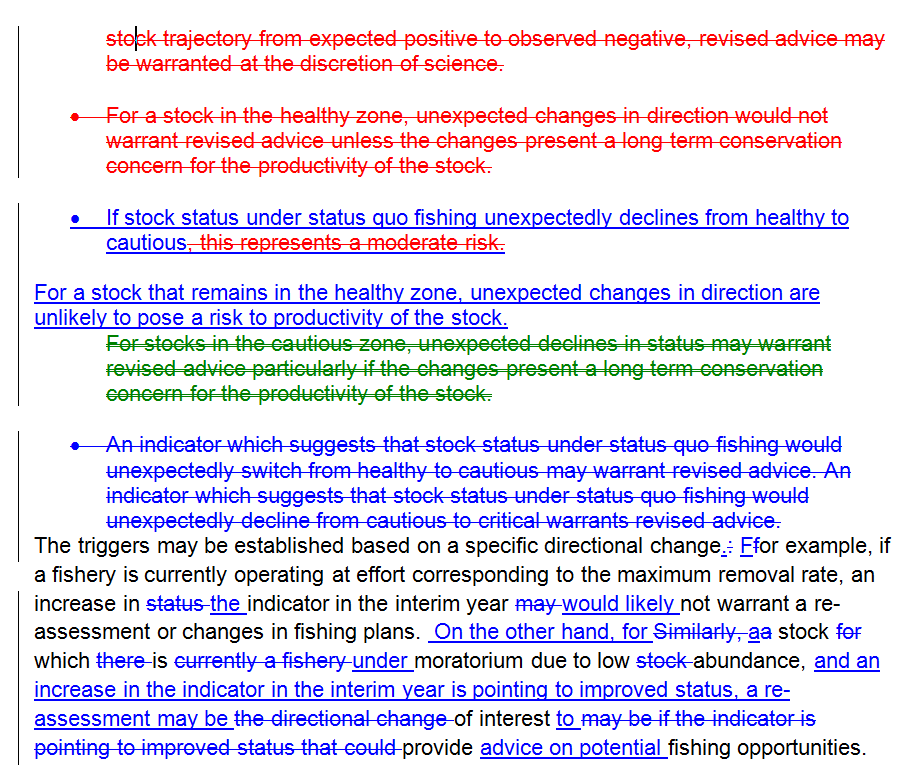
\includegraphics[
        width=\textwidth,
        height=0.8\textheight,
        keepaspectratio]
        {figures/interim.png}
  %\vspace{-3mm}
  %\caption{\tiny\url{https://www.reddit.com/user/NegativePitch}}
  \end{figure}
}

\frame{\frametitle{Relying on one person (e.g.~me) who holds up a project}

Often we have to work on other things, but our collaborators may have time.

  \centering
  \begin{figure}
    
\includegraphics[
        width=\textwidth,
        height=0.8\textheight,
        keepaspectratio]
        {figures/procEmail.png}
  %\vspace{-3mm}
  %\caption{\tiny\url{https://www.reddit.com/user/NegativePitch}}
  \end{figure}
}

\frame{\frametitle{Cluttering up directories}

We want to keep old versions in case we have to go back, but then ...

  \centering
  \begin{figure}
    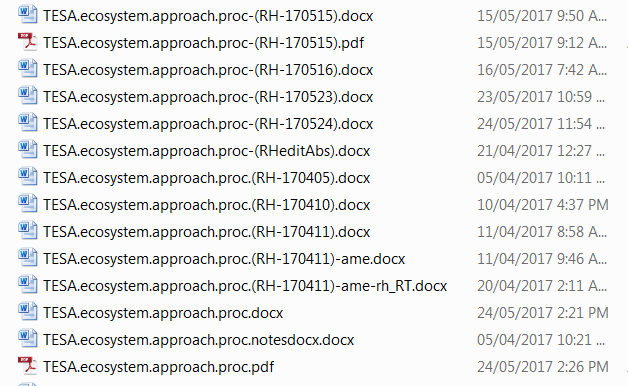
\includegraphics[
        width=\textwidth,
        height=0.8\textheight,
        keepaspectratio]
        {figures/EAversions.png}
  \end{figure}
}


 
\end{document}

\section{Creating/Cloning}
\frame{\frametitle{Creating a new repository}
  \bi
    \item Sign into your \gh\ account, click on the
      \emph{Repositories} tab, and press the \emph{New} button.
    \item Give your repository a name. I like to use small letters and dashes
      between words.
    \item Check \emph{Initialize this repository with a README}.
    \item Leave \emph{Add .gitignore} and \emph{Add a license}
      set to \emph{None}.
    \item Click \emph{Create repository}.
  \ei
}

\frame{\frametitle{Cloning your new repository}
  \bi
    \item Once you have created a repository on \gh, copy the URL
      of the repository.
    \item Open the \gs\ and run the following command to clone your repository:
      \lstinline{git clone URL REPO-NAME}\\
      where:\\
      \bi
        \item \lstinline{URL} is the url of your newly created repository. You
          can paste the \lstinline{URL} into the command line (on Windows) by
          pressing the right mouse button.
        \item \lstinline{REPO-NAME} will be the name of the directory to be
          created.
      \ei
  \ei
  \bigskip
  You should now have a subdirectory called \lstinline{REPO-NAME}. Enter that
  directory:\\
  \lstinline{cd REPO-NAME}
}

\frame{\frametitle{Windows only: Storing your credentials}
  When you push your changes to \gh, the \gs\ will ask you for your username
  and password every time. This is annoying, so issue the following command,
  and it will only ask you the first time. After that your credentials will be
  stored and you won't need to enter them again. You need to do this for each
  repository you clone.\\
  \bigskip
  \lstinline{git config --global credential.helper wincred}
}

\section{Committing new files}
\begingroup
\small
\frame{\frametitle{Copy and commit \emph{.gitignore}}
  \bi
    \item Copy the \emph{.gitignore} file from the git-course directory and
      paste it into your newly cloned directory. You can edit this to suit
      the project, as there is a different \emph{.gitignore} file for each
      project.
    \item Check the status of your repository: \lstinline{git status}
    \item You will see that the new file \emph{.gitignore} has not been
      staged for commit. It is an \emph{Untracked file}. You need to add any
      new files to be committed by using the \lstinline{git add} command:\\
      \lstinline{git add .gitignore}
    \item Make a commit for the changes:\\
      \lstinline{git commit -a -m "Added .gitignore"}\\
      or use the alias:\\
      \lstinline{git com "Added .gitignore"}\\
      the commit message should be a useful message saying what the commit
      encapsulates.
    \item Push the commit to \gh: \lstinline{git push}
    \item Check the \gh\ webpage and see your commit and that the file
      has been uploaded.
  \ei
}
\endgroup

\frame{\frametitle{Adding multiple files at once - slide 1}
  Often you add multiple files or a new directory with files in it. In
  these cases, when you run \lstinline{git status} or the alias
  \lstinline{git s}, you will see a large listing of files. Files can
  be added at once, by simply adding the directory.
  \bi
    \item Add a new directory to your repository, using your normal method.
      Call it \lstinline{test}.
    \item Add a couple of new test files to that directory called
      \lstinline{test1.r} and \lstinline{test2.r}. Put some example text
      in each and save them.
    \item On the command line, check the status:\\
      \lstinline{git status}\\
      or use the alias:\\
      \lstinline{git s}
    \item You will see a listing showing the \emph{test} directory in
      \emph{Untracked files}. To add the files in preparation for a commit,
      issue the command:\\
      \lstinline{git add test}
  \ei
  \bigskip
  Continued...
}

\frame{\frametitle{Adding multiple files at once - slide 2}
  \bi
    \item Check the status of the repository again:
      \lstinline{git status} or \lstinline{git s}
    \item It will now show a \emph{new file} in \emph{Changes to be committed}
    \item Commit the changes:\\
      \lstinline{git commit -a -m "Added new files to test directory."}\\
      or use the alias:\\
      \lstinline{git com "Added new files to test directory."}
    \item Push the changes to \gh:\\
      \lstinline{git push}
    \item Check the \gh\ webpage and see your commit and that the files
      have been uploaded.
  \ei
}

\frame{\frametitle{Renaming files}
  \bi
    \item You can rename any files the normal way you do that such as in the
      Windows file explorer.
    \item Once you've renamed your files, check the repository status:\\
      \lstinline{git status}\\
    \item You will see that the files you renamed need to be added again.
      Do this the same way you added them in the first place. You can also
      add a whole directory again and \gs\ is smart enough to only add the
      renamed files.
    \item Check the status again:\\
      \lstinline{git status}\\
      It will show that the file(s) were renamed.
    \item Make a commit:\\
      \lstinline{git com "Renamed files x, y, and z"}\\
    \item Push the commit:\\
      \lstinline{git push}
  \ei
}

\frame{\frametitle{The \emph{.gitignore} file}
  Each repository can have one \emph{.gitignore} file, in the root directory
  of the repository. This file has names of files or wildcard names such as
  \lstinline{*.dvi} or \lstinline{*.nav} that will be completely ignored by
  \gs. Many compilers make temporary files, the names of which should be added
  to this file to avoid adding these files when adding whole directories
  using commands such as \lstinline{git add test}.\\
  \bigskip
  This is important as you will clutter up your repository and have to spend
  time cleaning it all up.\\
  \bigskip
  Anytime you run the command \lstinline{git status} and there are files listed
  that you don't want added to the repository, you should add them or a
  wildcard template encapsulating them to the \emph{.gitignore} file.
}

\section{Branches}
\frame{\frametitle{Branching overview}
  When you want to add some new code to your project, but don't want to break
  what is already there, you create a new branch. When creating a new branch,
  your starting point is identical to the branch you were in when you created
  the new one.\\
  \bigskip
  Once you have completed your work in the new branch and are satisfied that
  everything is working correctly, you merge the changes into your master
  branch (or any other branch you wish).\\
  \bigskip
  You can also push branches to \gh\ if you feel the branch is going to be a
  longer term project and/or if there are going to be multiple collaborators
  on that new branch.\\
  \bigskip
  It is a good idea to commit all changes before creating a new branch, as
  local changes which haven't been coimmitted will appear in the new branch
  as well.
}

\frame{\frametitle{Creating a new branch}
  \bi
    \item To create a new branch based off the branch you are currently on:\\
      \lstinline{git checkout -b BRANCH-NAME}\\
      or use the alias:\\
      \lstinline{git cb BRANCH-NAME}\\
      You will be automatically placed in the new branch, and commits
      you make will now occur in the new branch.
    \item To view all local branches:\\
      \lstinline{git branch}
    \item to switch to another branch:\\
      \lstinline{git checkout BRANCH-NAME}\\
      or use the alias:\\
      \lstinline{git co BRANCH-NAME}\\
  \ei
}

\frame{\frametitle{Deleting branches}
  \bi
    \item To delete a branch that you are not currently in:\\
      \lstinline{git branch -d BRANCH-NAME}\\
    \item To delete the branch you are currently in, switch to another branch
      first, (e.g. master) and then delete the branch:\\
      \lstinline{git co master}\\
      \lstinline{git branch -d BRANCH-NAME}\\
    \item If you have changes in the branch, you will not be allowed to delete
      it. If you want to forcibly delete it, discarding your changes, use:\\
      \lstinline{git branch -D BRANCH-NAME}\\
      \textbf{Warning - you won't be able to get any of those changes back
        once you do this.}
  \ei
}

\frame{\frametitle{Merging branches}
  \bi
    \item To merge the changes from a branch into another branch:
      \bn
        \item Change to the branch you want to merge into, typically master:\\
          \lstinline{git co master}
        \item Merge the branch into master:\\
          \lstinline{git merge BRANCH-NAME}
      \en
    \item If there was a merge conflict, you must fix it at this point. This
      will be covered later in the section about merging remotes, which
      follows the exact same method.
    \item If you are done with that branch for good, delete it so you don't
      have unused branches hanging around:\\
      \lstinline{git branch -d BRANCH-NAME}
  \ei
}

\frame{\frametitle{Pushing branches to \gh}
  If you want to push the branch up to \gh, i.e. so others can fetch it and
  edit it, you need to be in the branch locally and:\\

  \lstinline{git --set-upstream origin BRANCH-NAME}\\

  \gs\ is somewhat smart, so if you forget this command and instead type:\\

  \lstinline{git push}\\

  while in the new branch, \gs\ will tell you the command you need.\\
  \bigskip
  Once you've done this for a branch, all you have to do to push future
  commits in this branch is:\\
  \lstinline{git push}\\
  \bigskip
  Check the \gh\ webpage to make sure your branch was pushed.
}

\frame{\frametitle{Deleting branches from \gh}
  To remove a branch entirely from \gh:\\
  \lstinline{git push origin --delete BRANCH-NAME}\\
  \bigskip
  The local branch will still exist, so if you want to delete that as well:\\
  \lstinline{git co master}\\
  \lstinline{git branch -d BRANCH-NAME}
}

\section{Remotes}
\frame{\frametitle{Remotes overview}
  Once you have created a repository on \gh\ and uploaded some files, you may
  want to start collaboration with others. To do this, send them the URL of
  your \gh\ repository, and ask them to \emph{Fork} it on \gh. Once they have
  done that and cloned your repository, everyone involved will need to add
  each other's repository as a \emph{remote} so that all changes can be merged.\\
  \bigskip
  Adding remotes has to be done once for each project. Once you have added
  someone, their remote information remains on your local computer. \gh\ has
  some smart programming, which detects merges between remotes and will keep
  track of the project and all its contributions.\\
  \bigskip
  The network graph is a great place to look at what has happened on a given
  repository.
}

\frame{\frametitle{Adding remotes}
  \bi
    \item Once everyone has \emph{Forked} on \gh, you must add each person as
      a \emph{remote}. They must also add everyone else as remotes. Everyone
      must trade URLs, and add each other person like this:\\
      \lstinline{git remote add REMOTE-NAME REMOTE-URL}\\
      where:\\
      \bi
        \item \lstinline{REMOTE-NAME} is a name you make up that you will
          remember. I use first initial followed by last name for everyone,
          so they have the same syntax. e.g.: cgrandin, aedwards, rforrest.
        \item \lstinline{REMOTE-URL} is the URL on \gh\ where the person's
          repository can be found. e.g.:\\
          \url{https://github.com/cgrandin/git-course}.
      \ei
    \item To view all remotes you have set up:\\
      \lstinline{git remote -v}\\
      or the alias:\\
      \lstinline{git r}
  \ei
}

\frame{\frametitle{Deleting or renaming remotes}
  \bi
    \item To delete someone as a remote:\\
      \lstinline{git remote delete REMOTE-NAME}\\
      where \lstinline{REMOTE-NAME} is the name you made up when you added them.
    \item To rename a remote:\\
      \lstinline{git remote rename OLD-NAME NEW-NAME}\\
      where \lstinline{OLD-NAME} is the name you made up when you added them and
      \lstinline{NEW-NAME} is the name you want to change it to.
    \item To see your changes, use:\\
      \lstinline{git remote -v}\\
      or the alias:\\
      \lstinline{git r}
  \ei
}

\section{Fetchching and merging remotes}
\frame{\frametitle{Fetching overview}
  Once you have set up your remotes, you can fetch other people's commits.
  Before continuing work on your project, you should always check \gh, and
  see if your collaborators have been working, and if so, what their commits
  were. At this stage you get a general idea of what has been done since
  you last looked at the repository. Once you have familiarized yourself with
  the changes in a broad sense, you will want to merge them into yours.\\
  \bigskip
  Find the most recent commit on \gh's \emph{Network Graph}. It will have
  one person's name associated with it. That is the person you will fetch
  and merge in.\\
  \bigskip
  There may be some disarray in the network graph, but you can just merge
  each person's repository into yours in succession if you wish, which
  will clean up the network graph.
}

\frame{\frametitle{Fetching other people's changes}
  To fetch someone's changes:\\
  \bigskip
  \lstinline{git fetch REMOTE-NAME}\\
  \bigskip
  where \lstinline{REMOTE-NAME} is one in the list of remotes you have set up.
  This command fetches everything in the person's repository, including
  all branches. Running this command does not affect your repository
  in any way. The fetch stores the information in a cache, awaiting
  your command to merge.
}

\frame{\frametitle{Comparing the fetched repository with yours}
  Once you've fetched someone's repository, you can exactly see what has
  changed compared to yours. This is called \emph{Diff-ing}.
  \bi
    \item To compare the changes in their master to yours (make sure you are in
      the master branch in \gs):
      \lstinline{git diff REMOTE-NAME/master}\\
      or using the \emph{Difftool} if you have it set up:\\
      \lstinline{git difftool REMOTE-NAME/master}
    \item This will show you exactly what changes to each file you are about
      to merge into your repository.
    \item In general, I use \emph{diff} if there are only minor changes
      and \emph{difftool} if there are more changes or if more than one file
      has been changed.
  \ei
}

\frame{\frametitle{Merging the fetched repository into yours}
  \bi
    \item To merge the fetched repository's master branch into yours:\\
      \lstinline{git merge REMOTE-NAME/master}\\
      note that the merge will happen in the branch you are currently in, so make
      sure you are in the \lstinline{master} branch.
    \item To merge other branches:\\
      \lstinline{git merge REMOTE-NAME/BRANCH-NAME}\\
      note that the merge will happen in the branch you are currently in, so make
      sure you are in the \lstinline{BRANCH-NAME} branch.
  \ei
  At this point, you will either be up-to-date, meaning there were no merge
  conflicts, or you will have one or more merge conflicts. If you are
  up-to-date, you need to push back to your repository to complete the merge
  step:\\
  \lstinline{git push}\\
  If you have conflicts, you need to fix them before continuing work.
}

\begingroup
\small
\frame{\frametitle{Dealing with merge conflicts}
  The merge message will tell you which files are conflicting. Open those
  files one by one, and you will see the conflicted section bracketed like the
  following:\\
  \bigskip
  \lstinline{<<<<<<< HEAD}\\
  Line(s) of text/code which are currently in your file.\\
  \lstinline{=======}\\
  Line(s) of text/code which are trying to merge in, but conflict.\\
  \lstinline{>>>>>>> BRANCH-NAME}\\
  \bigskip
  where \lstinline{BRANCH-NAME} is the name of the branch you are trying to
  merge in from the previously-issued command:\\
  \lstinline{git merge BRANCH-NAME}\\
  All you do is remove the bracketing lines, the \lstinline{=======} line,
  and choose one of the line(s) of text/code to keep, or edit the line(s)
  to be something else entirely. Once you are done fixing each conflicted file,
  you need to commit the merge conflict and push the result:\\
  \lstinline{git com "Merge conflict resolved."}\\
  \lstinline{git push}
}
\endgroup

\frame{\frametitle{Dealing with merge conflicts - mergetool}
  You can also use a mergetool such as DiffMerge to fix the conflicts. It is
  easier in that it will open a new session for each conflict and place you
  at the correct place. You won't have to see the bracketing markers and the
  files will be edited by the mergetool to what you want. If you want to try
  the mergetool, after a merge conflict message, run:\\
  \lstinline{git mergetool}\\
  \bi
    \item The left panel is what is in the branch you are in when you called
      the merge command.
    \item The middle panel is what you will end up with once finished.
    \item The right panel is what is in the branch you are trying to merge
      in.
  \ei
  Once finished, click the X to close and the next conflicted file will pop
  up in a new session of DiffMerge. Once all conflicts have been resolved,
  issue a commit and push to complete to merge:\\
  \lstinline{git com "Merge conflict resolved."}\\
  \lstinline{git push}
}

\frame{\frametitle{\gh\ - Add collaborators}
  If your \gh\ repository is public, anyone can post an issue. If you want
  someone to be able to:
  \bi
    \item Set assignees to issues
    \item Receive notifications when you reply to their issue
  \ei
  You need to add them as a collaborator. Select the \emph{Settings} tab and
  then the \emph{Collaborators} button. Type their \gh\ username in and send
  them an invitation to collaborate.
}

\section{Stashing}
\frame{\frametitle{Stashing overview}
  If you are in the middle of working on something, but you need to change
  branches for some reason, you can \emph{stash} your changes and apply
  them back later. Let's say you are working in the master branch. To
  stash all changes in master:\\
  \lstinline{git stash}\\
  then change branches, and do whatever you like. To get those changes back,
  switch back to master:\\
  \lstinline{git co master}\\
  and apply the stashed changes:\\
  \lstinline{git stash pop}\\
  Note that nothing is committed, this just lets you put on hold your work
  in progress and come back to where you left off.
}

\frame{\frametitle{Stashing - make it into a branch}
  If you leave a stash for awhile and have made commits since the stash,
  then try to reapply it, you may get conflicts. The best way to apply a stash
  if you have modified things since you stashed is to let git create a branch
  for the stash, which you can then look at and edit if you wish before merging
  back into your master or other working branch:\\
  \bigskip
  \lstinline{git stash branch BRANCH-NAME}\\
  \bigskip
  where \lstinline{BRANCH-NAME} is the name you want to call the new branch.
  You can then merge this branch in as outlined in the merging slides and
  resolve conflicts in the same way as with remotes or other local branches.
}

\section{Undoing things}
\frame{\frametitle{Changing the commit message in the last commit}
  If you make a commit, then realize that your message had a spelling error,
  or needed more information in it, you can change the commit message:\\
  \bigskip
  \lstinline{git commit --amend -m "Correct message."}\\
  \bigskip
  This only works on the last commit. You can't change any other commit message
  using \emph{amend}.\\
  If you already pushed the commit before realizing that the message needs
  modification, do this:\\
  \bigskip
  \lstinline{git push --force}\\
  \bigskip
  after making the amendment to the commit message. You can also add more files
  before issuing the amendment commit and those files will be added to the commit
  you are amending. You can't add changes to file content this way though, you'll
  need to do another commit for that.
}

\frame{\frametitle{Undoing a commit}
  If you make a commit followed by other commits, then realize you want to undo
  the earlier commit, you use \emph{revert}:\\
  \bigskip
  \lstinline{git revert HASH}\\
  \bigskip
  where \lstinline{HASH} is the hash for the commit you want to undo. It is the
  20-byte string that appears with the commit.\\
  e.g.: \lstinline{1ef1da5659a4b147562b155ffb6289811adab36b}\\
  \gs\ is smart enough that you only need the first five or so digits:\\
  \bigskip
  \lstinline{git revert 1ef1d}\\
  \bigskip
  It is important to make a lot of commits, each with only small changes.
  You can only revert the whole commit, not parts.
}

\frame{\frametitle{Undoing changes not yet committed}
  If you've made a mess in your working directory and you want to change
  everything back to the way it was on the last commit:\\
  \bigskip
  \lstinline{git reset --hard HEAD}\\
  \bigskip
  If you've messed up a single file and just want that one file to go back
  to the way it was on the last commit:\\
  \bigskip
  \lstinline{git checkout HEAD file/to/restore.r}\\
  \bigskip
  Warning - running these commends will delete the changes you have made.
  Since you have not committed any changes, they will be lost. Make sure
  you are certain you don't need the changes before running these commands.
  If you aren't sure if you need the changes again in the future, use
  \lstinline{git stash} instead.
}


\frame{\frametitle{\lstinline{git merge} gone wrong - which is the HEAD?}
  \centering
  \begin{figure}
    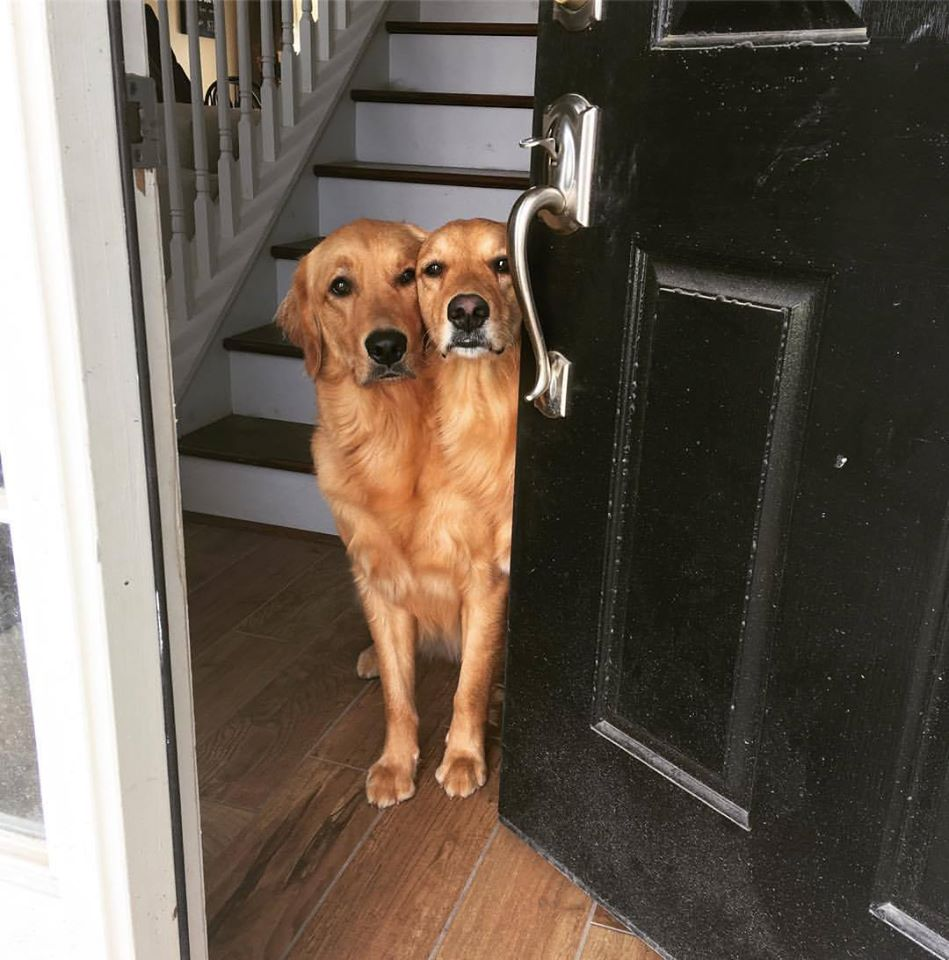
\includegraphics[
        width=\textwidth,
        height=0.8\textheight,
        keepaspectratio]
                    {figures/git-merge-failed-dogs}
  \vspace{-3mm}
  \caption{\tiny\url{https://www.reddit.com/user/NegativePitch}}
  \end{figure}
}

%% Git tower webpage:
%% https://www.git-tower.com/learn/git/ebook/en/command-line

%% Dog pic:
%% https://www.reddit.com/user/NegativePitch
%% http://i.imgur.com/zxm6UAh.jpg

\end{document}
